%% grundlagen.tex
%% $Id: grundlagen.tex 28 2007-01-18 16:31:32Z bless $
%%

\chapter{Background \& Related Work}
\label{ch:Background}

\section{Sensing with Earables}
Earables belong to the class of wearables and are a type of wearable device that is worn in or around the ears. 
They typically have a number of sensors that allow them to collect data about the wearer's physiology and activity. 
The most common sensors in earables include accelerometers, gyroscopes, and heart rate monitors. These sensors can be used to track the wearer's movements, monitor their heart rate, and provide other types of health data.
% TODO: Now link the paper from Röddiger and exend with summary of this paper

\section{Ear-based temperature measurement}
Ear-based temperature measurement uses a sensor to measure the temperature of the ear canal. 
The approach has a number of advantages over other measurement positions.
First, it is an non-invasive measurement procedure, which allows measurement nearly inside the body with the least amount of hematoma.
Second, the measurement is much more promising compared to other non-invasive alternatives, where many factors can contribute to falsify the final result \cite{asdf}. % TODO: modify citation

\subsection{Core Body Temperature}
Core body temperature is the temperature of the body's internal organs, such as the heart, liver and brain and is commonly used indicator of the human health and endurance performance.
Unlike the body core temperature, the body surface temperature is more easily influenced by the ambient temperature and therefore cannot reflect the changes inside the body as well as the body core temperature.
Core body temperature can be measured invasively rectally, orally (oesophagus), in the pulmonary artery (with the use of a catheter) or in the urinary bladder \cite{moranCoreTemperatureMeasurement2002a}. 
These types of measurement are uncomfortable for a person. 
In addition, because of this, it is not possible to take a measurement over a long period of time.

Body temperature can also be measured non-invasive.
This can be done on the axilla, the tympanic membrane, and the body surface \cite{moranCoreTemperatureMeasurement2002a}.
The tympanic membrane is a thin membrane that separates the middle ear from the external auditory canal. 
The artery called the external carotid artery runs near the external auditory canal and radiates heat, which is why measuring the temperature at the eardrum has a promising chance of determining body temperature \cite{yeohRevisitingTympanicMembrane2017}.

% TODO: \cite{yeohRevisitingTympanicMembrane2017} liefert in der introduction einiges zum thema blut temperatur und relevanz zu core body temperature

% TODO: \cite{ComparisonPulmonaryArtery}
% TODO: \cite{kimComparisonBilateralEardrum2022}
% TODO: \cite{childsTympanicMembraneTemperature1999}

\subsection{Core Body temperature vs skin temperature}

\subsection{2 grobsortierungen: optisch vs thermal resistor}
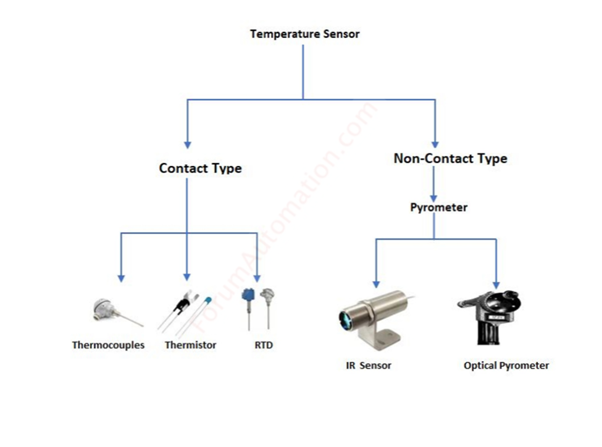
\includegraphics[scale=0.7]{thesis-doc/images/introduction/temp_sensor_types.png}
\subsubsection{optisch (Infarot)}
sendet lichtsprektrum, bestimmt anhand dessen die temperatur

\subsubsection{thermal resistor}
 widerstand, ändert widerstand nach temperature
 
\section{Analysis}
\subsection{Analysis based on body temperature}
\subsubsection{Fever}
\subsubsection{Circadian rhythm}
\subsubsection{...}

\subsection{Analysis based on temperature changes}
\subsubsection{...}